\chapter{Archipel Project}
    \section{Introduction}
Archipel repose totalement sur libvirt comme API de gestion des machines virtuelles. De fait, l'outil
s'impose d'être de plus haut niveau. Pour la gestion des utilisateurs, on peut directement utiliser un
serveur XMPP existant pour authentifier les personnes.

    \section{Architecture}
L'utilisation d'un serveur XMPP peut sembler étrange. L'application devra envoyer et recevoir des
informations avec les hyperviseurs et les machines virtuelles. Plutôt que de réécrire un n-ième protocole,
de l'implémenter, de devoir le débugger et le sécuriser, l'équipe d'Archipel avec XMPP a fait le choix de la
réutilisation. Ce protocole est défini par des RFC, et possède de nombreuses implémentations.
\begin{center}
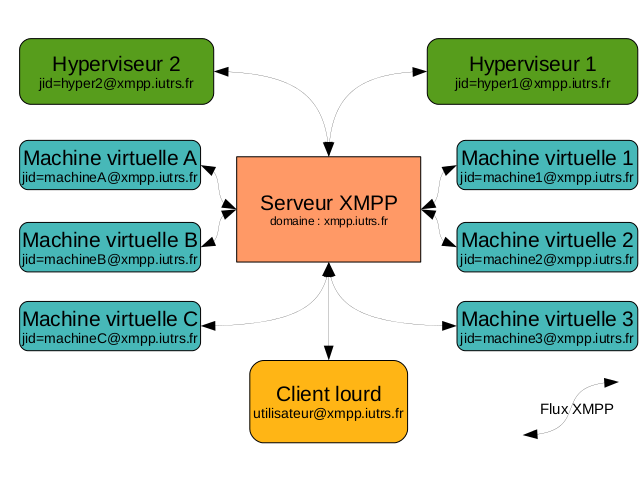
\includegraphics[width=10cm,height=7cm]{images/archi_archipel.png}
\begin{quote}llustration 1: Flux de messages entre les différentes entités\end{quote}
\end{center}

Il suffit donc d'avoir un client adapté pour les hyperviseurs et pour les machines virtuelles. Les machines
virtuelles, à un instant donné étant localisées sur un serveur, c'est au niveau de l'hyperviseur que
reposera la création des n instances de clients pour chacune des n machines virtuelles. Au niveau de
l'application de l'utilisateur, il y a également un client XMPP pour que les messages soient transmis aux
entités.\newline
En terme logiciel, un agent est installé sur chaque hyperviseur. Cet agent est scindé en deux parties :\newline
\begin{itemize}
 \item une incluant un client XMPP chargé de se connecter au serveur XMPP pour lui signaler sa présence.
 \item l'autre, plus complexe, est chargée de créer autant d'agents qu'il y a de machines
 virtuelles définies, chacun de ces agents intègre également un client XMPP.\newline
\end{itemize}

Du coté du client utilisateur, l'interface intègre un client XMPP. Toutes les communications bénéficient
donc des fonctionnalités du serveur XMPP, par exemple le roster (liste des contacts autorisés) qui donne
une certaine sécurité dans les dialogues entre entités. On « ajoute » donc un contact dans son roster, qui
peut être soit une machine virtuelle ou un hyperviseur. Lorsque dans l'interface client, on demande un
démarrage de la VM (« Virtual Machine », en français machine virtuelle), un stanza (un message XMPP)
est envoyé vers le serveur XMPP. Celui-ci vérifie que l’émetteur est dans le roster du destinataire, et lui
transmettra alors le message s'il est autorisé. L'agent, coté machine virtuelle, va recevoir ce message et
l'interpréter, donc lancer via l'API libvirt le signal start .\newline
Les agents, qu'il s'agisse de ceux liés à un hyperviseur ou à une machine virtuelle, exploitent la librairie
libvirt via le binding python. En particulier, c'est la partie events de libvirt qui est utilisée. De cette
manière, même si une interaction parallèle est effectuée sur les hyperviseurs (par exemple, l'utilisation de
virsh ou de virt-manager pour démarrer une entité, ajouter un nouveau réseau, ou créer une nouvelle VM
par un script), les agents seront informés et pourront remonter le nouvel état via un message XMPP.
Ce choix laisse la porte ouverte à une intégration fine dans un système existant : si vous aviez vos
propres scripts virsh pour créer des machines virtuelles, l'adoption d'Archipel ne vous force nullement à
renoncer à votre travail déjà en place !

    
    \section{Haute disponibilité et montée en charge}
Dans les solutions de gestions d'hyperviseurs, un critère souvent retenu est la Haute Disponibilité (HA).
Mais tout le monde ne met pas les mêmes éléments derrière ces mots. En terme de HA au niveau des
machines virtuelles, Archipel se repose complètement et uniquement sur libvirt. Au niveau d'Archipel lui
même, la haute disponibilité concerne l'échange des messages entre les entités, donc la haute
disponibilité du serveur XMPP lui même. Une utilisation d'une solution cluster de serveurs XMPP répond
donc à la demande. Ce mode cluster permet aussi de se rassurer au niveau de la montée en charge du
serveur car la multiplication des VM et des hyperviseurs va augmenter le nombre de stanza échangés.\newline
Au niveau des messages échangés, la notification de toutes les entités n'est pas nécessaire, ni voulue,
pour des raisons de charge de messages. Une solution consisterait à stocker du coté de l'agent, les
entités et les messages qu'elles doivent recevoir, mais il faudrait alors maintenir des états. L'architecture
a recours à un mécanisme très intéressant du coté du serveur XMPP. Il s'agit de la partie PubSub (PUBlish-
SUBscribe) : cela fonctionne comme les groupes de multicast au niveau réseau IP. Les entités qui
souhaitent diffuser des informations à plusieurs entités publient via une entrée dans le service PubSub du
serveur, et les entités qui souhaitent recevoir les messages pour cette entrée s'y abonnent. Ainsi, c'est
encore une fois le serveur XMPP qui va faire le travail de diffuser aux entités abonnées les messages. Cela
donne un flux optimal de messages, et simplifie la programmation des agents.\newline

    \section{Sécurité}
Dans une telle plate-forme, la gestion de la sécurité est importante. L'utilisation de XMPP en tant que
protocole permet déjà d'être rassuré sur l'intégrité des messages échangés : XMPP est issue d'un
processus de validation et de standardisation via les RFC et est implémenté depuis de nombreuses
années.\newline
La sécurité qui permet de savoir quel utilisateur peut dialoguer avec une entité repose d'abord sur le
roster de celle-ci, car comme le roster est stocké coté serveur XMPP, c'est sans doute la meilleure solution
qui puisse être retenue. Il est donc possible de définir clairement quel utilisateur peut dialoguer avec une
machine virtuelle ou un hyperviseur donnés, et également de savoir qui a accès à une entité donnée.
Archipel va encore plus loin dans la gestion de la sécurité. Comme ce sont des stanza qui définissent les
demandes entre les entités, et que cela se traduit par des appels à l'API de libvirt, un filtrage coté agent
est en place, il permet d'autoriser ou non certaines actions. Ainsi, actuellement, 110 rôles possibles sont
définis et il est possible d'attribuer à un utilisateur, l'accès ou non à chacun de ces rôles. Par exemple, on
peut donner à un webmestre, le droit d’accéder à la « console VNC » de sa machine virtuelle, ainsi que
l'action start et stop. Ou à un développeur, le droit de prendre des instantanés d'une machine virtuelle, et
de les restaurer.\newline
Dans un soucis de séparer les utilisateurs des entités machines virtuelles et hyperviseurs, on peut aller
encore plus loin (et s'intégrer encore mieux dans le système d'information). Les serveurs XMPP sachant
dialoguer ensemble, via une autorisation explicite au niveau du serveur pour autoriser le S2S (Server to
Server ), il est possible d'utiliser un autre serveur XMPP existant pour les utilisateurs (comme cela, ils
peuvent utiliser par exemple une authentification liée à leur ENT). Les messages transitent alors par les
deux serveurs successivement avant d'arriver aux entités coté Archipel.\newline
En terme de sécurité, là encore, Archipel se base sur l'existant, et ajoute de la finesse dans la délégations
de droits.\newline

    \section{Fonctionnalités}
Archipel étant encore jeune, les fonctionnalités les plus évidentes ont été mises en place. Le système de
module permet d'ajouter aisément de nouvelles fonctions. Tout ce qui est nécessaire à un travail
quotidien existe.\newline
Actuellement, la plupart des fonctions disponibles via l'interface virt-manager sont déjà en place :
définition d'une nouvelle VM, manipulations du réseau et du stockage, accès à la console VNC, gestions
des snapshots, etc... Les opérations de migration sont également prises en charge. Les nouvelles
possibilités sont celles qu'on attend d'un logiciel de management d'hyperviseurs : reporting sur l'état de
hyperviseur, création de nouvelles machines à partir de flux RSS (VMCast), planifications de taches,
gestions des droits des différents utilisateurs, création d'une machine avec détection automatique du
serveur le moins chargé, etc... Les développeurs sont pleins d'idées, il même est prévu, par exemple, un
module de facturation !\newline
La mise en place d'Archipel est très simple : il faut installer un serveur XMPP avec une configuration
correcte, puis installer sur chaque agent, un agent écrit en python. Cet agent, une fois correctement
configuré, va se cloner pour s’exécuter pour toutes les machines virtuelles, et va joindre le serveur XMPP.
A partir de ce moment là, Archipel est exploitable. Les machines virtuelles déjà en place bénéficient des
fonctionnalités d'Archipel (sauf au niveau de la gestion disque et migration). On ne peut pas faire
beaucoup plus simple.\newline
Et pour couronner le tout, l'application client n'est pas un client lourd standard. Tout le client est en fait
une application HTML5, en Javascript. C'est ce qui déconcerte généralement les premiers utilisateurs : il
n'y a pas de serveur web où l'application s’exécute. Il faut juste un serveur web pour stocker les fichiers
(dans certains cas et avec le navigateur chrome uniquement, il est même possible d’exécuter l'application
depuis les fichiers stockés en local). Une fois chargé, c'est uniquement le Javascript qui fait tourner tout le
client. Le framework utilisé est Cappuccino, qui donne un aspect très MacOsX. Le client XMPP y est
également intégré. Donc quand vous utilisez votre client, vous dialoguez directement vers le serveur
jabber !

    \section{Conclusion}
Archipel s'intègre bien dans le courant UNIX : Keep It Simple, Stupid. D'autres solutions préfèrent
construire des monstres d'infrastructure. Se baser sur libvirt permet de s'assurer d'avoir la main via virsh
ou virt-manager, en cas de soucis de client, d'agent, ou même si le serveur XMPP pose problème, cela
permet de dormir tranquille.\newline
Cependant Archipel a encore quelques faiblesses. A force d'exploiter la robustesse de XMPP, peu de
serveurs implémentent tout ce qui est nécessaire. Ejabberd est pour l'instant le seul serveur XMPP qui est
recommandé. Archipel a également mis en évidence un certain nombre de bugs dans libvirt. En particulier
la gestion de Xen et de Vmware dans libvirt reste problématique, et rend inopérant Archipel (la balle est
dans le camp des développeurs de libvirt). Enfin Archipel propose déjà un certain nombre de
fonctionnalités qui le rend largement utilisable, et il reste de la place pour l'innovation.\newline
La mise en place n'affecte pas l'existant, elle est relativement aisée à effectuer, ce qui permet de faire
une migration en douceur.\newline
Enfin, Archipel répond a un besoin récurrent mais simple : pouvoir donner un accès restreint à certaines
machines pour certains utilisateurs. La délégation de droits est simple à effectuer. De plus, avec une
interface conviviale et sans client lourd, en HTML5, il n'y a pas de problème pour donner un accès à des
non informaticiens.

    \section{Installation et configuration sur tous les noeuds}
	\subsection{Installation et configuration de jabber}
Archipel a besoin de ejabberd comme XMPP serveur (Pour le moment seulement ejabberd supporte efficacement le protocole XMPP pour les
besoin de Archipel). 

Installation de ejabberd par les dépôts:
\begin{lstlisting}
  apt-get install ejabberd
\end{lstlisting}
\begin{quotation}
Note, il faut une version suppérieure ou égale à la 2.1.0, si la dristribution ne permet pas cela il faut changer de distribution.
\end{quotation}

Archipel a besoin des modules ejabberd suivants pour fonctionner:

\begin{itemize}
\item mod\_admin\_extra (installer avec les packages de ejabberd)
\item ejabberd\_xmlrpc (module optionel)
\end{itemize} 
 
\begin{quotation}
Si il y a besoin de compiler les modules faire ce qui suit, sinon passer cette étape.
\end{quotation}

\subsection{Installation de l'environement de erlang}
\begin{lstlisting}
apt-get install subversion erlang-dev erlang-xmerl build-essential erlang-tools python-setuptools
\end{lstlisting}

\subsection{Obtention des module ejabberd}
\begin{lstlisting}
cd /usr/local/src
svn checkout http://svn.process-one.net/ejabberd-modules/
\end{lstlisting}

\subsection{librairie Erlang xmlrpc}
Cette librairie n'est pas inclue dans le package Debian il faut donc faire cela:
\begin{lstlisting}
cd /usr/local/src
wget http://ejabberd.jabber.ru/files/contributions/xmlrpc-1.13-ipr2.tgz
tar -xzf xmlrpc-1.13-ipr2.tgz
cd xmlrpc-1.13/src
vi Makefile
\end{lstlisting}

Puis:
\begin{lstlisting}
make
\end{lstlisting}

Finalement, copier la librairie dans le répertoire contenant les librairie erlang:
\begin{lstlisting}
cd /usr/local/src
cp -a xmlrpc-1.13 /usr/lib/erlang/lib/
\end{lstlisting}

\subsection{Compilation du module ejabberd\_xmlrpc}
Compilation de ebin pour le module jabberd\_xmlrpc module:
\begin{lstlisting}
cd /usr/local/src/ejabberd-modules/ejabberd_xmlrpc/trunk
./build.sh
cp ebin/ejabberd_xmlrpc.beam /usr/lib/ejabberd/ebin/
\end{lstlisting}
Il est possible que quelques warning apparaissent: 
\begin{lstlisting}
gen_mod, gen_mod.erl:176: Warning: the regexp module is deprecated (will be removed in R15A); use the re module instead...
\end{lstlisting}
Mais tout va bien.

\subsection{Compilation et installation de mod\_admin\_extra}
mod\_admin\_extra peut être inclus dans le package ejabberd, so you certainly don't need to build it

\subsection{configuration de jabber}
Le fichier de configuration Debian par défaut (ejabberd.cfg)  est une configuration pour le serveur de chat de base 
(cequi est bien pour un serveur de chat) mais archipel a besoin d'options plus avancées pour être un vrai serveur 
complet XMPP. il faut donc supprimer le fichier de base:
\begin{lstlisting}
rm / etc / ejabberd / ejabberd.cfg
\end{lstlisting}
Puis copier l'exemple suivant\newline 
(https://github.com/primalmotion/Archipel/wiki/Ejabberd\%3A-Configuration) 
dans un nouveau fichier nommé / etc / ejabberd / ejabberd.cfg, 
et remplacer l'occurrence de nom de domaine complet par votre nom de domaine 
réel (et aussi éventuellement mettre à jour le chemin de la certificat TLS).\newline

Puis démarrer ejabberd:
\begin{lstlisting}
  ejabberdctl start
\end{lstlisting}

Attendre 10 secondes puis vérifié si c'est démarré:
\begin{lstlisting}
/opt/sbin/ejabberdctl status
> The node ejabberd@FQDN is started with status: started
> ejabberd 2.1.8 is running in that node
\end{lstlisting}

Il faut créer un compte administrateur:
\begin{lstlisting}
ejabberdctl register admin votre.domaine.com votrepass
\end{lstlisting}

\section{Installation de l'agent archipel}
Pour l'installer depuis le package python:\newline
En tant que root, lancé depuis l'hyperviseur:
\begin{lstlisting}
easy_install archipel-agent
\end{lstlisting}

Depuis le version téléchargée sur le site\newline
 (http://nightlies.archipelproject.org/latest-archipel-client.tar.gz)
\begin{lstlisting}
easy_install apscheduler xmpppy sqlalchemy numpy
cd /chemin/du/repertoire/ArchipelAgent/
./buildAgent -d
\end{lstlisting}

Depuis les sources:\newline
Valable seulement avec un clone du dépôt:
\begin{lstlisting}
easy_install apscheduler xmpppy sqlalchemy numpy
cd /path/to/clone/ArchipelAgent/
./buildAgent -d
\end{lstlisting}

\subsection{Post installation}

Finalisation de  l'installation

Pour finir l'installation de Archipel:
\begin{lstlisting}
# archipel-initinstall
\end{lstlisting}

\subsection{Personaliser l'installation}

Le fichier de configuration de archipel ce trouve dans:\newline
/etc/archipel/archipel.conf il faut l'adapter en fonction du système. 
Pour plus d'information ce renseigner sur:\newline
(https://github.com/primalmotion/Archipel/wiki/Installation\%3A-archipel-agent\%27s-configuration-file)


Si vous avez juste installer le server ejabberd, il faut crée les suivant pubsub nodes pour le stockage.Il suffit de lancer:
\begin{lstlisting}
archipel-tagnode --jid=admin@FQDN --password=YOURPASSWORD --create
archipel-rolesnode --jid=admin@FQDN --password=YOURPASSWORD --create
archipel-adminaccounts --jid=admin@FQDN --password=YOURPASSWORD --create
archipel-vmparkingnode --jid=admin@FQDN --password=YOURPASSWORD --create
[OPTIONAL] archipel-vmrequestnode --jid=admin@FQDN --password=YOURPASSWORD --create
\end{lstlisting}

Si vous voulez utiliser la caractéristique de vmparking, Il faut déclérer l'hyperviseur comme éditeur. 
Pour ce faire, lancer pour chaque hyperviseurs:
\begin{lstlisting}
archipel-vmparkingnode --jid=admin@FQDN --password=YOURPASSWORD -a hypervisor_jid@FQDN
\end{lstlisting}


\subsection{Lancement de l'agent}

Et enfin pour lancer /etc/archipel/archipel.conf faire:
\begin{lstlisting}
/etc/init.d/archipel start
ejabberdctl connected_users
\end{lstlisting}

vous devriez avoir une réponse comme: hypervisor@votre.domain.com
\begin{lstlisting}
Update Archipel Agent
Update PyPi installation
\end{lstlisting}

Pour mettre à jour archipel quand un noeud est ajouté:
\begin{lstlisting}
# easy_install -U archipel-agent
# /etc/init.d/archipel restart
\end{lstlisting}

\section{Installation du client archipel}
Pour installer le client il suffit de récupérer l'archive du client d'archipel\newline
(http://nightlies.archipelproject.org/latest-archipel-client.tar.gz)
puis la décomprésser dans le répertoire du server web et d'y accédé par le navigateur.
